\begin{figure*}[t]
    \centering
    \begin{tikzpicture}[font={\tiny},]   
         %% CNN branch
        \node(input) at (-5.5, 0) {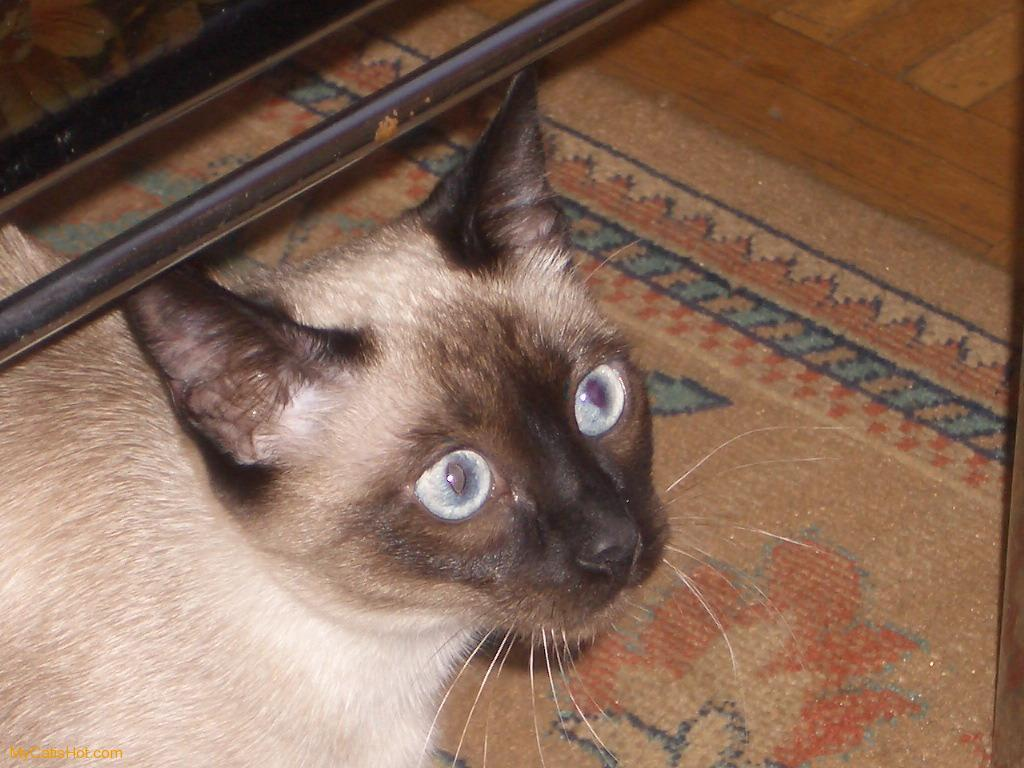
\includegraphics[width=.12\textwidth]{Images/Method/input.jpg}};
        \node[] at (input.north) {\footnotesize Input image $\vx$};
        \node[draw, trapezium, rotate=-90,trapezium angle=75, align=center] (bbne) at (-2.5,0) {\rotatebox{90}{\parbox{2cm}{\centering{\footnotesize Backbone}}}};
        \node[draw, align=center] (wv) at (0.1, -0.8) {$w^V$};
        \node[draw, align=center] (wk) at (-0.95, -0.8) {$w^K$};
        \node[shape=circle,draw=black] (mm1) at (-0.95, -1.5) {$\times$};
        \node[](empt1) at (6.5, 0){};
        \node[draw, rotate=90, align=center] (class) at (7,0) {\footnotesize Classifier};
        \node(logit) at (7.75, 0) {\small$\vy$};
        % %%% CLS stream
        \node[align=center](clsin) at (-4, -1.5) {{\footnotesize[CLS]}};
        % \node[draw, align=center](CA0) at (-2.5, -1.5) {{\footnotesize CA-0}, \\$d_\ell:$\\64*BE};
        % \node[draw, align=center](CA1) at (-0.5, -1.5) {{\footnotesize CA-1}, \\$d_\ell:$\\128*BE};
        % \node[draw, align=center](CA2) at (1.5, -1.5) {{\footnotesize CA-2}, \\$d_\ell:$\\256*BE};
        % \node[draw, align=center](CA3) at (3.5, -1.5) {{\footnotesize CA-3}, \\$d_\ell:$\\512*BE};
        % \node[draw, align=center](CA4) at (5.5, -1.5) {{\footnotesize CA-4}, \\$d_\ell:$\\512*BE};

        % %% CNN backbone
        \node(empt0) at (-4.48, 0) {};
        \draw[->] (empt0.center) -- node {} (bbne);
        \draw[->] (bbne.east) -| node {} (wv);
        % \draw[->] (res1) -- node {} (res2);
        % \draw[->] (res2) -- node {} (res3);
        % \draw[->] (res3) -- node {} (res4);
        % \draw[->] (res1) -- node {} (res2);
        % \draw[->] (res2) -- node {} (res3);
        % \draw[->] (res3) -- node {} (res4);
        % \draw[->, blue, dashed] (res4) -- node {\blue{\normalsize//}} (class);
        % \node[](GAP) at (6,0.25) {\footnotesize\blue{$\gap$}};
        % \draw[->] (class) -- node {} (logit);
        % %% CLS Stream
        \draw[->] (clsin) -- node {} (mm1);
        % \draw[dashed, ->] (res0.north) -|node {} (CA0);
        % \draw[->] (CA0) -- node {} (CA1);
        % \draw[dashed, ->] (res1.north) -|node {} (CA1);
        % \draw[->] (CA1) -- node {} (CA2);
        % \draw[dashed, ->] (res2.north) -|node {} (CA2);
        % \draw[->] (CA2) -- node {} (CA3);
        % \draw[dashed, ->] (res3.north) -|node {} (CA3);
        % \draw[->] (CA3) -- node {} (CA4);
        % \draw[dashed, ->] (res4.north) -|node {} (CA4);
        % \draw[-] (CA4.east) -| node {} (empt1.center);
        % \draw[->] (empt1.center) -- node {} (class);        
        % \path[->] (CA4.east) edge[bend right,left] node {} (class.north);
        % \path [->] (B) edge[bend right=60] node {$1$} (E); 
    \end{tikzpicture}
    \caption{Cross Attention Stream applied to ResNet-based architectures. Given a CNN backbone $f(\cdot)$, we replace global average pooling with  the introduction of a global representation [CLS] learned with the inclusion of the cross attention attention stream.}
    \label{fig:fig_method}
\end{figure*}